\documentclass[10pt,a4paper]{article}

\renewcommand{\familydefault}{\sfdefault}
\usepackage{helvet}
\usepackage[hidelinks]{hyperref}
\usepackage{xparse}
\usepackage{graphicx}
\usepackage{hanging}

\usepackage[utf8]{inputenc}
\inputencoding{utf8}
\usepackage[official]{eurosym}

\usepackage[
	top=1cm,
	bottom=1cm,
	left=1cm,
	right=1cm,
]{geometry}

\begin{document}
	\pagenumbering{gobble}
	\clearpage
	
	\noindent\begin{minipage}[t]{0.62\textwidth}
		{\Huge DAVID STUTZ}\\[8px]
		{\LARGE Informatiker}
		\vskip 6px
		
		Informatik fasziniert mich. Mit einem Schwerpunkt auf Bilderkennung- und verarbeitung sowie machinellem Lernen, kombiniere ich Theorie mit den interessantesten Anwendungen der heutigen Welt.
	\end{minipage}
	\hspace{0.025\textwidth}
	\begin{minipage}[t]{0.2\textwidth}
		\raggedleft
		David Stutz
		davidstutz@web.de\\
		\href{http://davidstutz.de}{davidstutz.de}\\
		\href{https://github.com/davidstutz}{github.com/davidstutz}
	\end{minipage}
	\hspace{0.005\textwidth}
	\begin{minipage}[t]{0.145\textwidth}
		\vskip -16px
		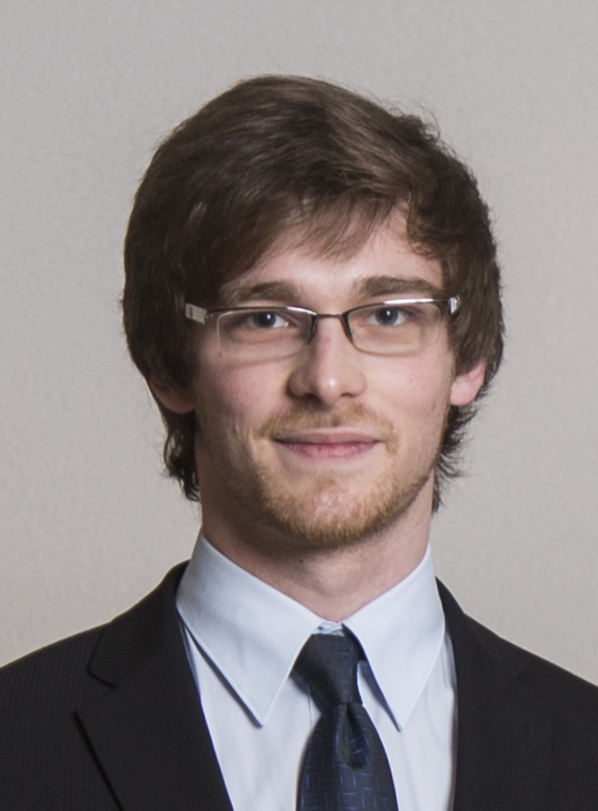
\includegraphics[scale=0.175]{photo}
	\end{minipage}
	\vskip 12px
	
	\noindent\begin{minipage}[t]{0.65\textwidth}
		\noindent{\LARGE BILDUNG}
		
		\vskip -6px
		\rule{\textwidth}{0.5px}
		\vskip 12px
		
		\noindent\begin{minipage}[t]{0.25\textwidth}\raggedleft
			10/2014 -- heute\\
			10/2011 -- 09/2014
		\end{minipage}
		\hspace{0.025\textwidth}
		\begin{minipage}[t]{0.725\textwidth}
			RWTH Aachen (Aachen, DEU)\\
			Master of Science, Informatik (Durchschnittsnote: 1,0)\\
			Bachelor of Science, Informatik (Abschlussnote: 1,1)\\
			{\footnotesize Bachelorarbeit: Superpixel Segmentation using Depth Information}\\
			{\footnotesize Schwerpunkte: Bildverarbeitung und -erkennung, Machinelles Lernen, Mustererkennung, Numerik}
		\end{minipage}
		\vskip 8px
		
		\noindent\begin{minipage}[t]{0.25\textwidth}\raggedleft
			1/2015 -- 5/2015
		\end{minipage}
		\hspace{0.025\textwidth}
		\begin{minipage}[t]{0.725\textwidth}
			Georgia Institute of Technology (Atlanta, USA)\\
			Austauschsemester, Informatik (Durchschnittsnote: 1,0)
		\end{minipage}
		\vskip 8px
		
		\noindent\begin{minipage}[t]{0.25\textwidth}\raggedleft
			8/2002 -- 3/2011
		\end{minipage}
		\hspace{0.025\textwidth}
		\begin{minipage}[t]{0.725\textwidth}
			Privates Gymnasium Calvarienberg (Ahrweiler, DEU)\\
			Abitur (Abschlussnote: 1,2)\\
			{\footnotesize Prüfungsfächer: Physik, Mathematik, Englisch, Erdkunde}
		\end{minipage}
		\vskip 12px
		
		\noindent{\LARGE ERFAHRUNG}
		
		\vskip -6px
		\rule{\textwidth}{0.5px}
		\vskip 12px
		
		\noindent\begin{minipage}[t]{0.25\textwidth}\raggedleft
			7/2016 -- 9/2016
		\end{minipage}
		\hspace{0.025\textwidth}
		\begin{minipage}[t]{0.725\textwidth}
			Microsoft Corporation (Dublin, IRL)\\
			Praktikant, Softwareentwicklung
		\end{minipage}
		\vskip 8px
		
		\noindent\begin{minipage}[t]{0.25\textwidth}\raggedleft
			4/2016 -- 6/2016
		\end{minipage}
		\hspace{0.025\textwidth}
		\begin{minipage}[t]{0.725\textwidth}
			MOBIS Parts Europe N.V. (Frankfurt a.M., DEU)\\
			Praktikant, Frontkamera für Fahrerassistenzsysteme\\
			{\footnotesize Entwicklung eines experimentellen Prototypen für Fußgänger-Detektion basierend auf aktueller Forschung im Bereich Deep Learning.}
		\end{minipage}
		\vskip 8px
		
		\noindent\begin{minipage}[t]{0.25\textwidth}\raggedleft
			5/2015 -- 3/2016
		\end{minipage}
		\hspace{0.025\textwidth}
		\begin{minipage}[t]{0.725\textwidth}
			Computer Vision Group, RWTH Aachen (Aachen, DEU)\\
			Studentische Hilfskraft\\
			{\footnotesize Evaluierung und Vergleich aktueller Algorithmen zur Generierung von Superpixeln.}
		\end{minipage}
		\vskip 8px
		
		\noindent\begin{minipage}[t]{0.25\textwidth}\raggedleft
			5/2015 -- 3/2016
		\end{minipage}
		\hspace{0.025\textwidth}
		\begin{minipage}[t]{0.725\textwidth}
			Fyusion Inc. (San Francisco, USA)\\
			Forscher und Entwickler\\
			{\footnotesize Entwicklung von Prototypen und Durchführung von Experimenten im Bereich Fußgänger-Detektion, Verfolgung von Geradenabschnitten, Verfolgung lokaler Bildmerkmale und statistische Clusteranalyse.}
		\end{minipage}
		\vskip 8px
	
		\noindent\begin{minipage}[t]{0.25\textwidth}\raggedleft
			10/2013 -- 1/2014\\
			4/2014 -- 9/2014
		\end{minipage}
		\hspace{0.025\textwidth}
		\begin{minipage}[t]{0.725\textwidth}
			MATHCCES, RWTH Aachen (Aachen, DEU)\\
			Studentische Hilfskraft\\
			{\footnotesize Leitung von Tutorien für ``Analysis für Informatiker'' und ``Mathematische Grundlagen~II''; wöchentliche Korrektur von Übungen; Korrektur der Klausur.}
		\end{minipage}
		\vskip 8px
		
		\noindent\begin{minipage}[t]{0.25\textwidth}\raggedleft
			1/2009 -- 3/2014\\
			10/2014 -- 4/2015
		\end{minipage}
		\hspace{0.025\textwidth}
		\begin{minipage}[t]{0.725\textwidth}
			RS Computer (Sinzig, DEU)\\
			Softwareentwickler\\
			{\footnotesize Entwicklung von Templates und Plugins für Content Managment Systeme wie CMSimple und Wordpress; Konzeption, Implementierung und Wartung individueller Web-Anwendungen auf Basis von PHP, Javascript und SQL für mittelständige Unternehmen.}
		\end{minipage}
		\vskip 8px
	
		\noindent\begin{minipage}[t]{0.25\textwidth}\raggedleft
			10/2009\\
			5/2011 -- 7/2011\\
			3/2012\\
			8/2012 -- 9/2012
		\end{minipage}
		\hspace{0.025\textwidth}
		\begin{minipage}[t]{0.725\textwidth}
			Fraunhofer FKIE (Wacthberg, DEU)\\
			Werkstudent\\
			{\footnotesize Entwicklung einer Web-Anwendung auf Basis von PHP und Kohana zur Verwaltung großer MySQL-Datenbanken und Durchführung komplexer Anfragen mittels SQL; Plugin-Entwicklung für Piwik mit Hilfe von JavaScript und PHP; Datenvisualisierung mittels d3.js.}
		\end{minipage}
		\vskip 12px
	\end{minipage}
	\hspace{0.035\textwidth}
	\begin{minipage}[t]{0.315\textwidth}
		
		\noindent{\LARGE PUBLIKATIONEN}
		
		\vskip -6px
		\rule{\textwidth}{0.5px}
		\vskip 12px
		
		{
		\hangpara{16px}{1}D. Stutz. \textit{Superpixel Segmentation: An Evaluation}. GCPR, 2015.
		\vskip 12px
		}
		
		\noindent{\LARGE STIPENDIEN}
		
		\vskip -6px
		\rule{\textwidth}{0.5px}
		\vskip 12px
		
		\noindent
		{\raggedright
		\hangpara{16px}{1}Accenture Future Technology Leader Program\\
		RWTH Bildungsfond\\
		RWTH Dean's List\\
		Hans Hermann-Voss Stipendium\\
		e-fellows.net Stipendium\\
		careerloft.de Stipendium\\
		\hangpara{16px}{1}Buchpreis der Deutschen Physikalischen Gesellschaft\\
		\hangpara{16px}{1}Teilnahme an der Deutschen Juniorakademie
		\vskip 12px
		}
		
		\noindent{\LARGE SPRACHEN}
		
		\vskip -6px
		\rule{\textwidth}{0.5px}
		\vskip 12px
		
		\noindent
		Deutsch (Muttersprache)\\
		Englisch (fließend)
		\vskip 12px
		
		\noindent{\LARGE KENNTNISSE}
		
		\vskip -6px
		\rule{\textwidth}{0.5px}
		\vskip 12px
		
		\noindent
		C++ (Boost, OpenCV)\\
		Python (OpenCV, Caffe, Numpy)\\
		MatLab\\
		PHP (Kohana, Wordpress)\\
		JavaScript (jQuery, d3.js)\\
		SQL\\
		HTML/CSS\\
		LaTeX (TikZ, PGFPlots)\\
		
		\noindent
		Microsoft Windows\\
		Linux (Ubuntu)\\
		Microsoft Office\\
		Git, Mercurial\\
	\end{minipage}
\end{document}